\documentclass[hyperref={colorlinks,citecolor=blue,linkcolor=blue,urlcolor=blue}]{beamer}

% For more themes, color themes and font themes, see:
% http://deic.uab.es/~iblanes/beamer_gallery/index_by_theme.html
%
\mode<presentation>
{
  \usetheme{Madrid}       % or try default, Darmstadt, Warsaw, ...
  % \usecolortheme{default} % or try albatross, beaver, crane, ...
  \usefonttheme{default}    % or try default, structurebold, ...
  \setbeamertemplate{navigation symbols}{}
  \setbeamertemplate{caption}[numbered]
} 

\usepackage[english]{babel}
\usepackage[utf8x]{inputenc}
\usepackage{chemfig}
\usepackage[version=3]{mhchem}

% On Overleaf, these lines give you sharper preview images.
% You might want to `comment them out before you export, though.
% \usepackage{pgfpages}
% \pgfpagesuselayout{resize to}[%
%   physical paper width=8in, physical paper height=6in]

% Here's where the presentation starts, with the info for the title slide
\title[]{RATIONING MEDICINE THROUGH BUREAUCRACY: AUTHORIZATION RESTRICTIONS IN MEDICARE \\ 
Brot-Goldberg et. al, 2023}
\author{Han Zhang}
\institute{UT Austin}
\date{}

\begin{document}

\begin{frame}
  \titlepage
\end{frame}

% These three lines create an automatically generated table of contents.
\begin{frame}{Background}
    \begin{itemize}
        \item Administrative costs make up a substantial portion of healthcare spending in the United States
        \item half of administrative effort is spent on activities that aim to reduce healthcare utilization and spending
        \item evaluate the trade-off between administrative burden for potential reductions in moral hazard and lower costs of insurance provision
        \item specifically, of prior authorization restrictions in healthcare, specifically focusing on their impact on drug utilization and healthcare costs
    \end{itemize}
    
\end{frame}
\begin{frame}{Innovation}
    \begin{itemize}
        \item comprehensive analysis of the effects of prior authorization on drug utilization using a large dataset and advanced statistical techniques
        \item examines the efficiency and equity implications of prior authorization policies, shedding light on their broader impacts on the healthcare system.
    \end{itemize}
\end{frame}
\begin{frame}{Literature}
    \begin{itemize}
        \item the bureaucratic ‘waste’ that has been the main focus of prior research (Casalino et al. 2009, Cutler et al. 2012, Gottlieb et al. 2018, Dunn et al. 2020) needs to be counterbalanced with the direct effects of bureaucratic activities.
        \item contributes to a broader literature on the trade-offs inherent in bureaucracy
        \item contributes to a literature on rationing mechanisms in health care
    \end{itemize}
\end{frame}

\begin{frame}{Outline}
  \tableofcontents

\end{frame}

\section{Prior Authorization Restrictions in Theory and Practice}
\begin{frame}{Prior Authorization Restrictions in Practice}
    \begin{itemize}
        \item  Prior Authorization Restrictions: insurers require approval from providers before covering certain medical services or prescription drugs 
       
        \item Purpose: ensures appropriate utilization of healthcare resources, control costs
        \begin{itemize}
            \item the responses to questions on the prior authorization forms explicitly transmit information about value to the patient from experts (physicians) to payers
            \item The physician’s willingness to complete the forms implicitly signals to the payer that the value of the drug or treatment to the patient is high enough to justify going through the process.
        \end{itemize}
    \end{itemize}
\end{frame}

\subsection{A Model of Prior Authorization Restriction}
\begin{frame}{A Model of Prior Authorization Restriction}
    \textbf{without} Prior Authorization Restriction
    \begin{itemize}
        \item $\triangle v_{id}=v_{id}-v_{i(-d)}$ the incremental value; $\triangle c_{id}$ the incremental cost
        \item consumer type $\theta \in [0,1]$
        \item The patient will receive the drug if $u(\theta_{id})\geq0$
        \item social welfare $$W(0)=\int_{\Theta_0} [V_d(\theta)-C_d(\theta)]d\theta $$, where  $\Theta_0 = \{\theta: u(\theta_{id}) \geq 0\}$
    \end{itemize}
\end{frame}
\begin{frame}{A Model of Prior Authorization Restriction}
    \textbf{with} Prior Authorization Restriction
    \begin{itemize}
       \item new choice utility function $u_A(\theta_{id})$
       \item administrative cost $a$
       \item social welfare $$W(1)=\int_{\Theta_1} [V_d(\theta)-C_d(\theta)]d\theta -a$$, where  $\Theta_1 = \{\theta: u_A(\theta_{id}) \geq 0\}$
    \end{itemize}
    Welfare Impact of Prior Authorization Restriction:
    $$W(1)-W(0) = -\int_{\Theta_M} V_d(\theta)+\int_{\Theta_M} C_d(\theta)d\theta -\int_{\Theta_1}a $$
    , where $\Theta_M = \Theta_0 \backslash \Theta_1 $
\end{frame}
\begin{frame}{Model: When Should Policymakers Restrict Drugs?}
    this model implies drugs under the restriction should be: 
    \begin{itemize}
        \item Optimizing Administrative Costs: few inframarginal users
        \item Addressing Moral Hazard: incremental value is low
        \item Ideal drugs for restriction are expensive, niche-branded drugs, particularly new entrants in established therapeutic classes
    \end{itemize}
    \begin{figure}
        \centering
        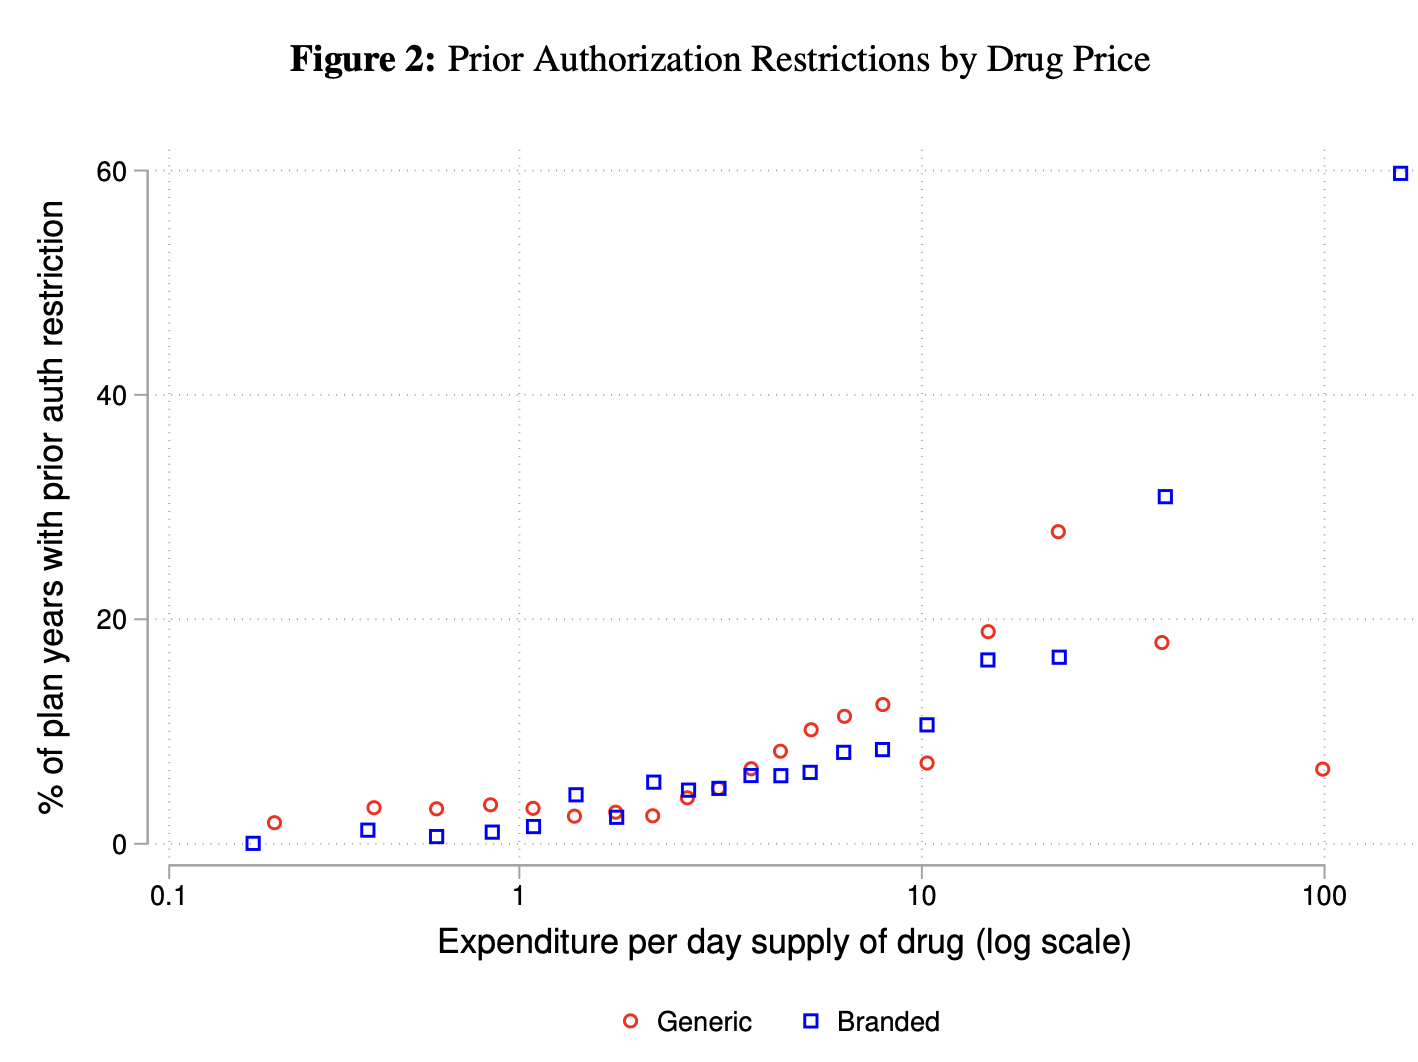
\includegraphics[width=0.5\linewidth]{fig2-price-restriction.png}
    \end{figure}
\end{frame}

\section{Setting \& Data}
% \subsection{Medicare Part D}

\subsection{Data}
\begin{frame}{Data}
    utilizes administrative datasets from the Centers for Medicare and Medicaid Services (CMS) from 2007 to 2015.

    \begin{enumerate}
        \item Beneficiary Demographics, Enrollment, and Choice Status
        \begin{itemize}
            \item tracks whether enrollment was initiated through active choice or the default auto-assignment mechanism. 
            \item allows us to observe the \textit{assigned} plan and the \textit{enrolled} plan for each beneficiary, even when the two differ.
        \end{itemize}
        \item Plan Characteristics 
        \item Formulary Data: drug-level, the set of drugs covered by each plan each year 
        \item Outpatient Prescription Drug Data
        \item Other Drug Information: rebates etc.
    \end{enumerate}
\end{frame}

\subsection{Sample Selection}
\begin{frame}{Data: Sample Selection}
    \begin{itemize}
        \item restriction to full Low Income Subsidy (LIS) Beneficiaries
        \begin{itemize}
            \item they effectively pay nothing out of pocket for covered drugs, making prior authorization the primary feature of the insurance contract that shapes drug demand
            \item they frequently face default rules which assign them to a randomly-chosen plan if they do not make an active plan choice
        \end{itemize}
        \item restrict to those who were automatically reassigned to a benchmark plan 
        \item data from the year before their reassignment to two years after reassignment
    \end{itemize}
\end{frame}

% \subsection{Prior Authorization in Medicare Part D}


\section{the Effect on Drug Utilization}
\begin{frame}{The Effect of Authorization Restrictions on Drug Utilization}
    the treatment effect of moving a drug from being covered with no restrictions to being covered with restrictions, all else equal. \\
    
    identification challenges: 
    \begin{enumerate}
        \item beneficiaries are free to choose plans, beneficiaries intending to take specific drugs may be inclined to avoid plans that restrict the drugs they want, introducing reverse causality between propensity to use a drug and whether a beneficiary faces prior authorization
        \item plans do not randomly select which drugs to restrict
    \end{enumerate}
   
\end{frame}
\begin{frame}{Effect of on Drug Utilization: Research Design}
 solutions: 
 \begin{enumerate}
     \item
     %   For beneficiaries who face random assignment to default plans, their assigned plan is, by construction, orthogonal to any underlying drug preferences of the beneficiary themselves. Therefore, we 
     restrict to \textit{only} beneficiaries who faced random assignment to default plans.
   \item use an indicator for whether the drug was restricted under the beneficiary’s \textbf{assigned plan} as an \textbf{instrument} for whether the drug was restricted under the beneficiary’s \textbf{enrolled plan}, for each beneficiary-drug pair
   \item rich controls: drug-by-market fixed effects; assigned-plan-by-market fixed effects; whether the drug was excluded in the enrolled plan; formulary status of substitutes
 \end{enumerate}

\end{frame}
\begin{frame}{Effect of on Drug Utilization: Research Design}
    estimating equations
    \begin{equation}
    \begin{aligned}
        Y_{idt} & =\beta_1Auth^{Enrolled}_{idt}+\beta_2 Excl^{Enrolled}_{idt}+\kappa_{dm(it)}+\lambda_{j(it)m(it)} \\
        &\gamma_1 Auth^{Sub,Assigned}_{j(it)dt} + \gamma_2 Excl^{Sub,Assigned}_{j(it)dt} + \nu_{idt}
    \end{aligned}
    \end{equation}
    \begin{equation}
        \begin{bmatrix}
    Auth^{Enrolled} \\
    Excl^{Enrolled}_{idt}
        \end{bmatrix}
        =
        \begin{aligned}
         & \delta_1Auth^{Enrolled}_{idt}+\delta_2 Excl^{Enrolled}_{idt}+K_{dm(it)}+\Lambda_{j(it)m(it)} \\
        &\Gamma_1 Auth^{Sub,Assigned}_{j(it)dt} + \Gamma_2 Excl^{Sub,Assigned}_{j(it)dt} + u_{idt}
        \end{aligned}
    \end{equation}
     $$$$
     where the utilization outcome is a binary indicator for whether the beneficiary filled the drug at least once in the year.
\end{frame}
\begin{frame}{Effect of on Drug Utilization: : Main Estimates}
    \begin{figure}
        \centering
        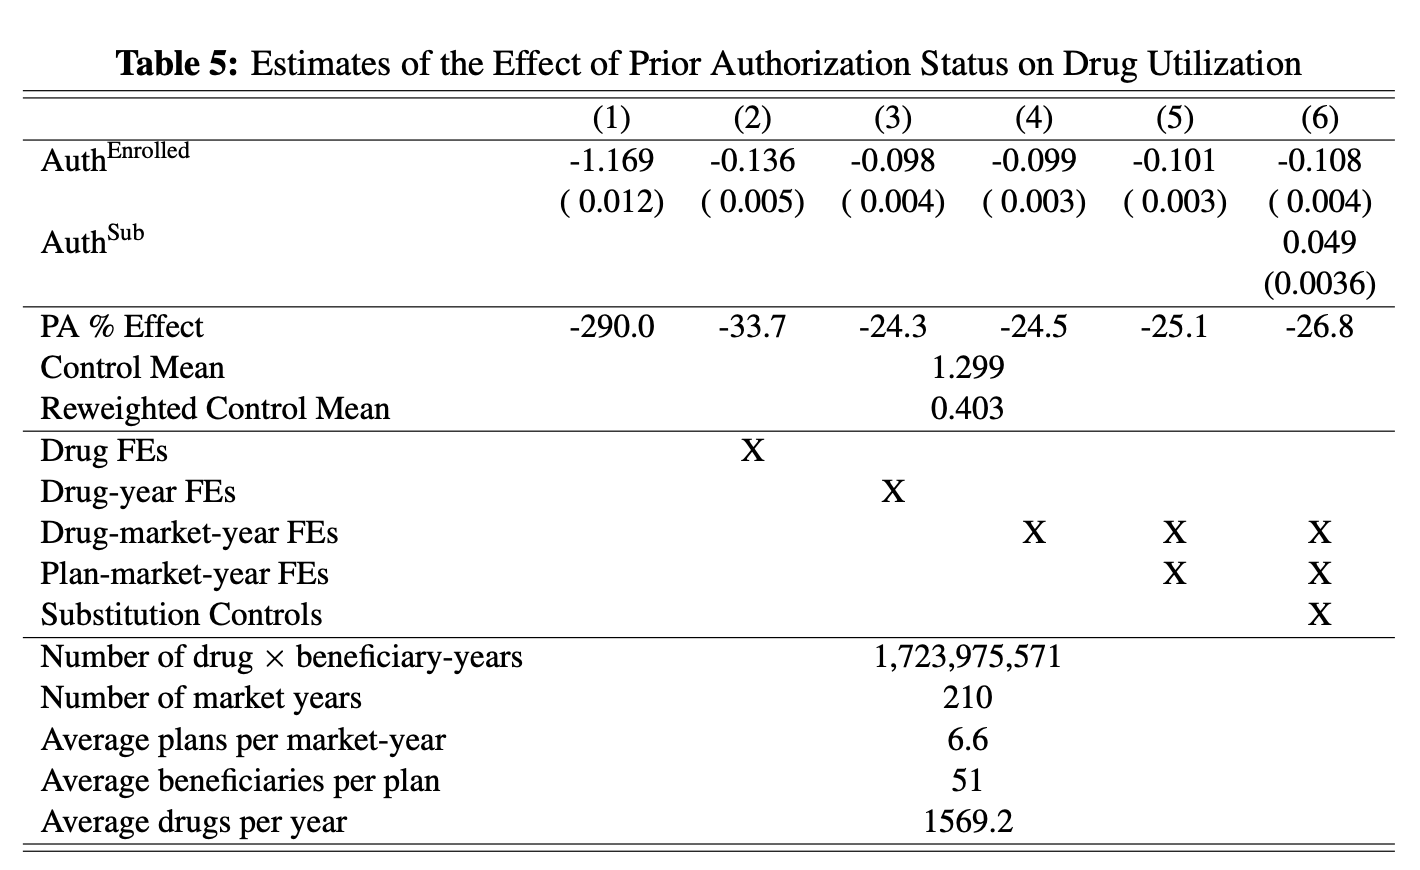
\includegraphics[width=0.7\linewidth]{tb5-2sls.png}
        \caption{\%PA effect = coefficient estimates divided by reweighted control mean}
    \end{figure}
\end{frame}
\begin{frame}{Effect of on Drug Utilization: Heterogeneous Effects}
    \begin{figure}
        \centering
        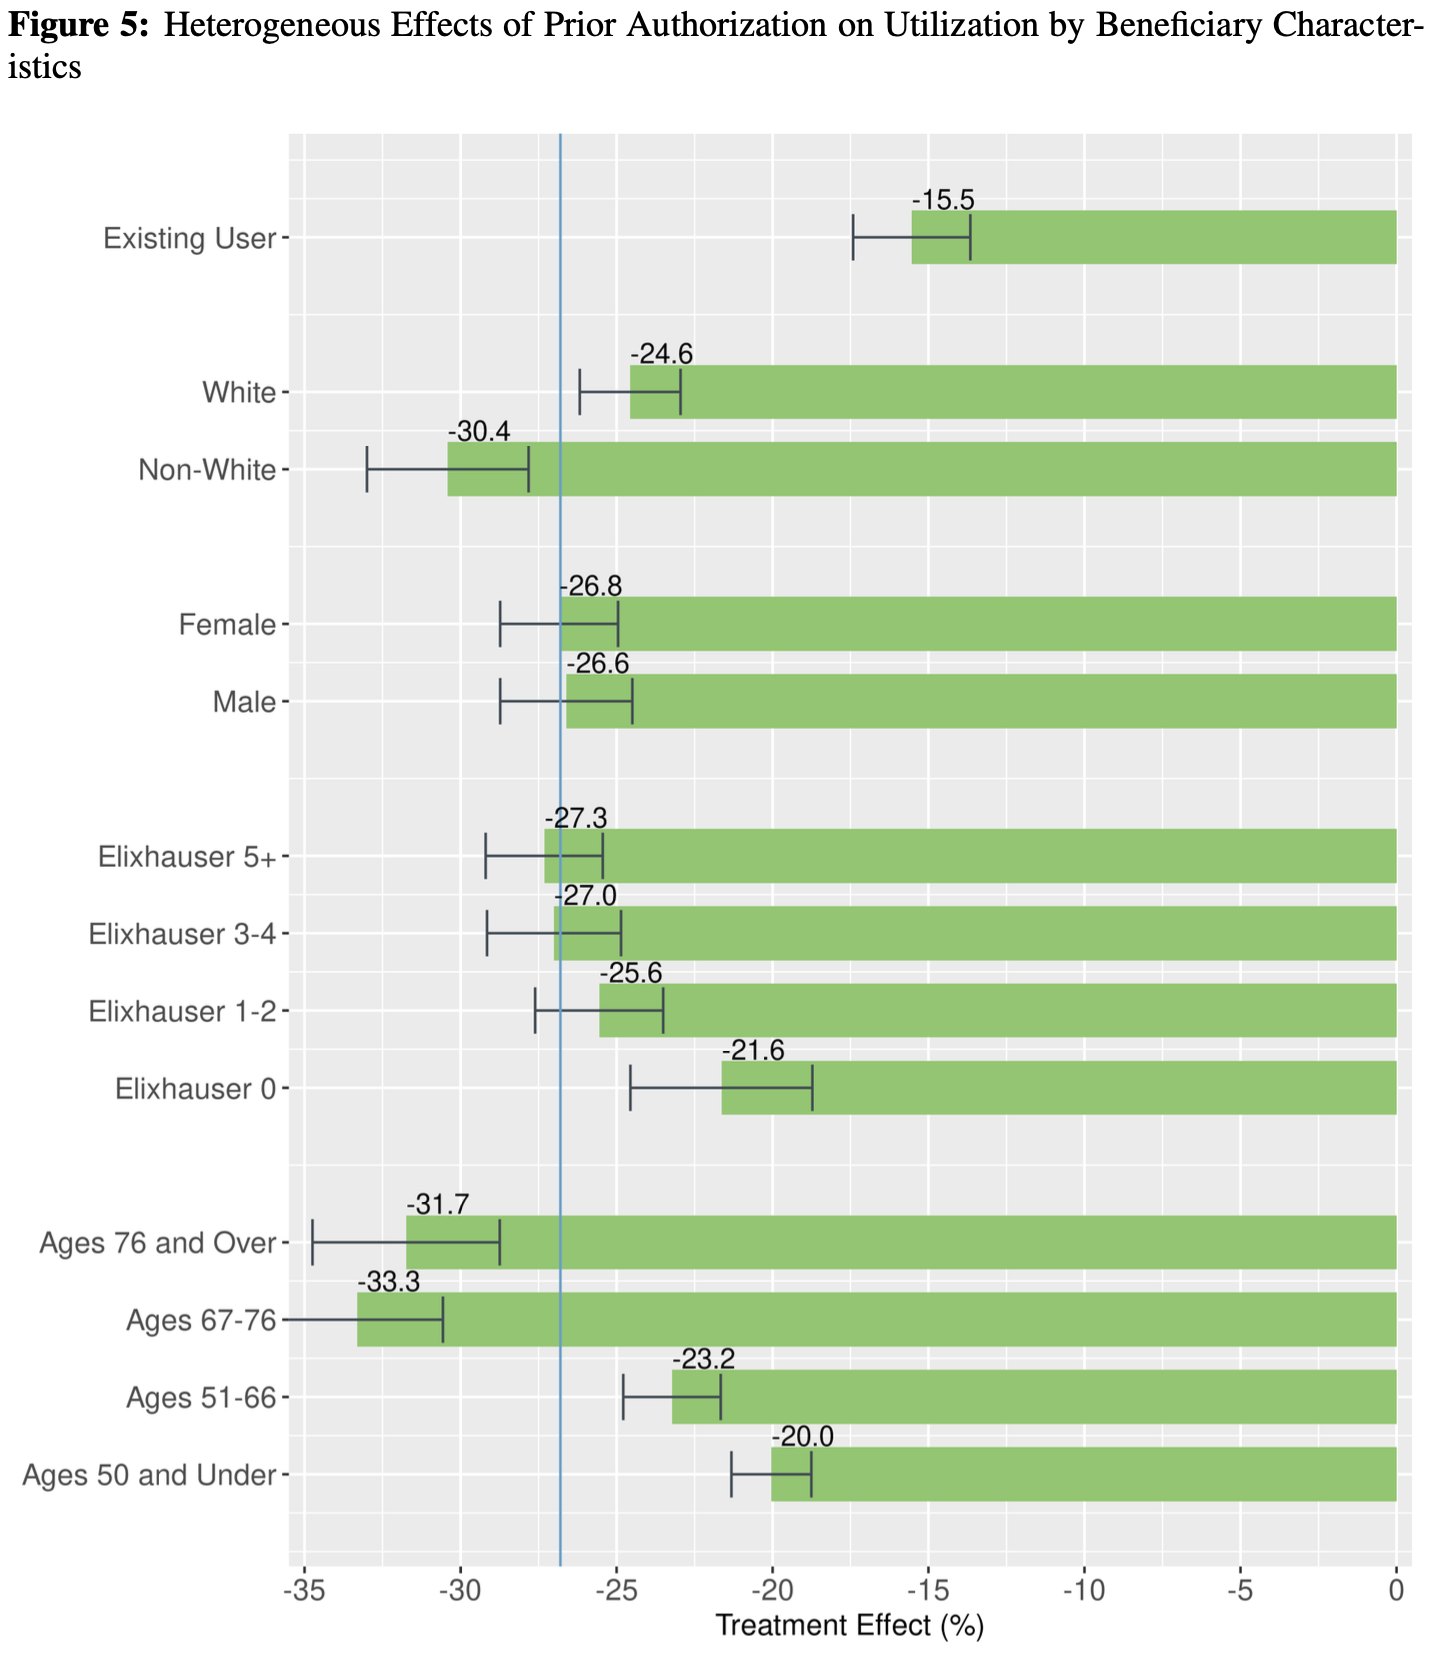
\includegraphics[width=0.5\linewidth]{fig5.png}

    \end{figure}
\end{frame}
\begin{frame}{Effect of on Drug Utilization: Heterogeneous Effects}
    \begin{figure}
        \centering
        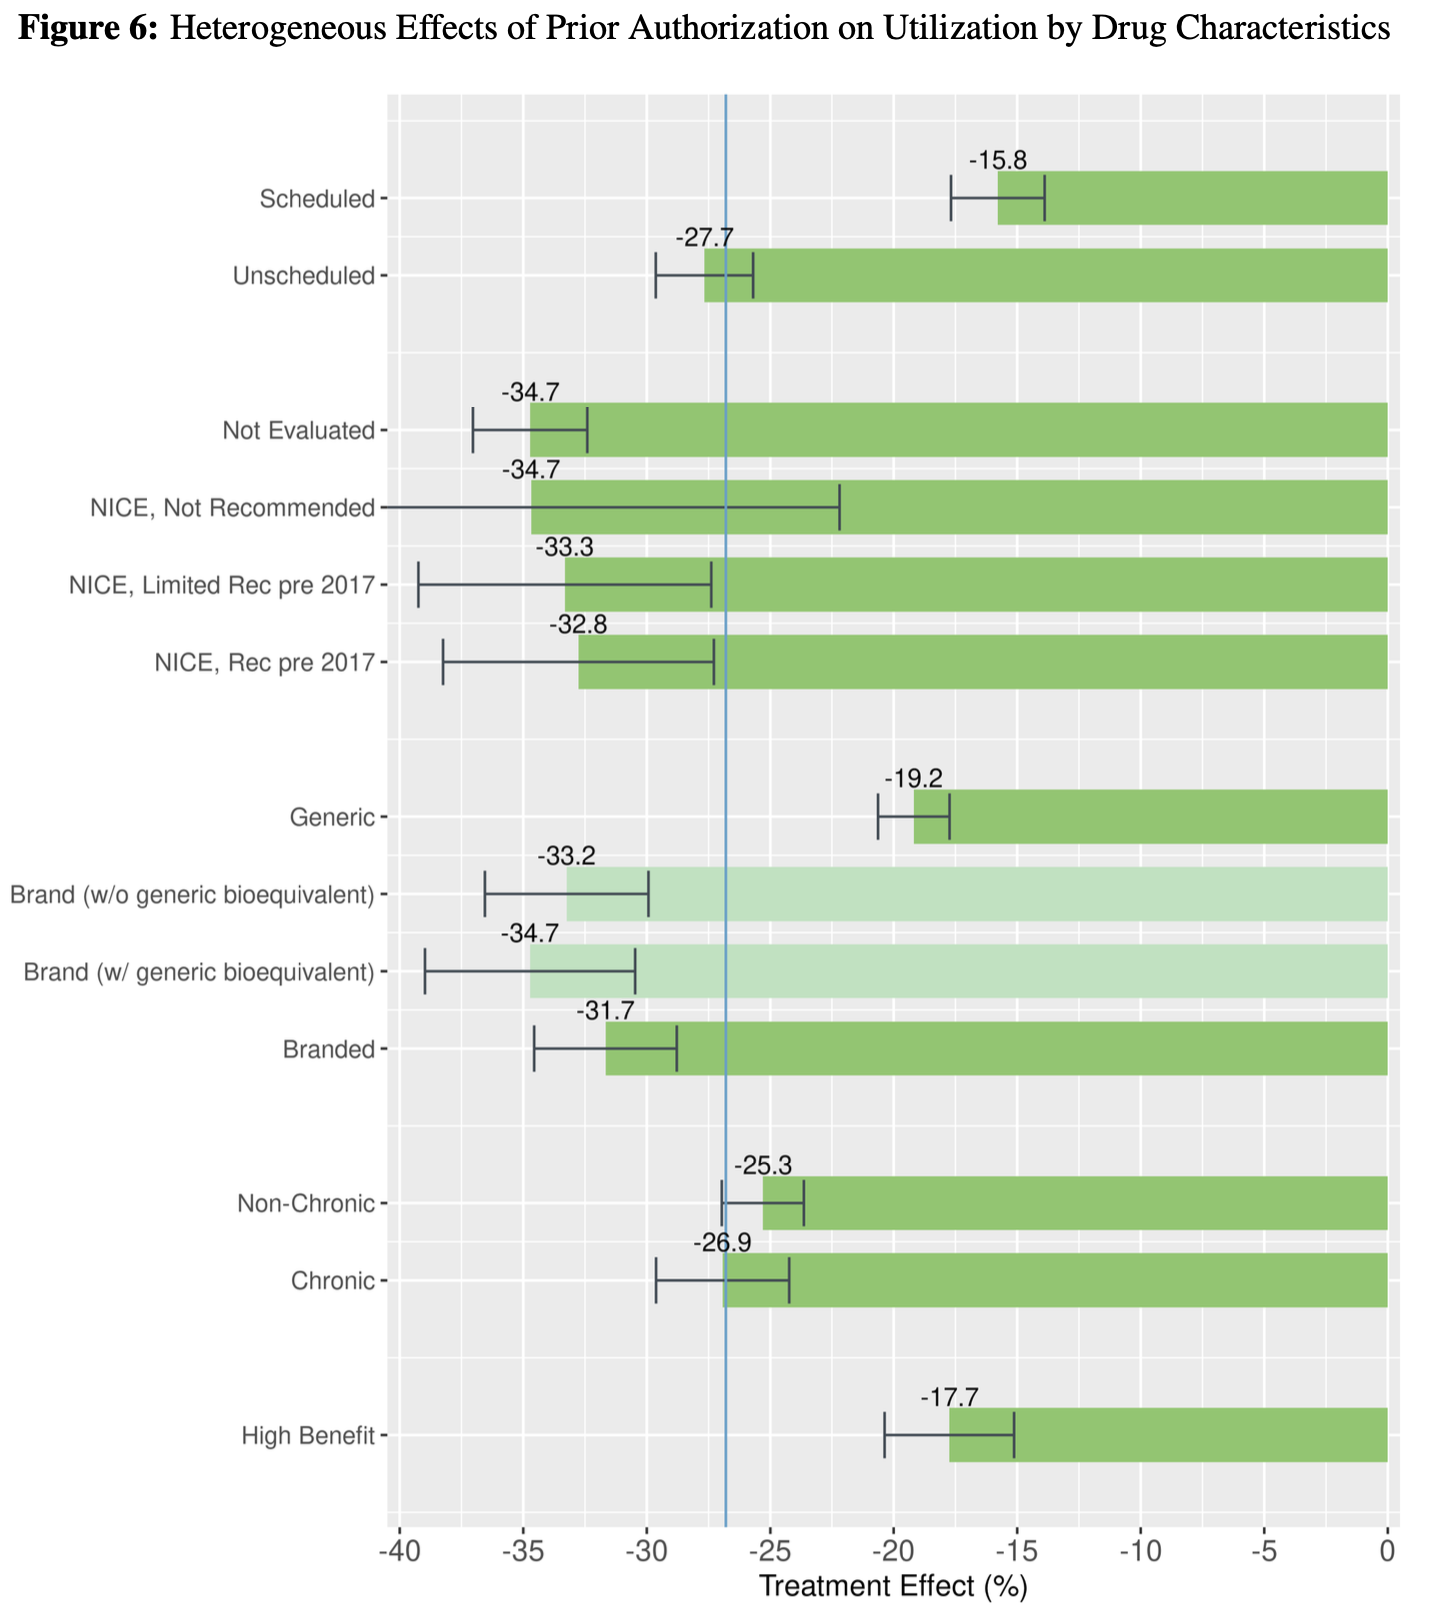
\includegraphics[width=0.5\linewidth]{fig6.png}
       
    \end{figure}
\end{frame}

\section{Substitution Patterns and Spending Effects}
\begin{frame}{Spending Effects: Estimating Substitution Patterns}
    a discrete choice of a single drug within a therapeutic class for a given year:
    $$u_{idt}= \underbrace{\beta_C Auth_{idt} + \delta_C Excl_{idt} + \kappa_{dm(it)}}_\text{$V_{idt}$} + \xi_{iCt}1\{d\neq 0\} + \lambda_{C\epsilon idt} $$
    which implies a nested logit demand system. The probability of taking a drug is
    $$P_{id}= \frac{\exp \frac{V_{idt}}{\lambda_C}(\Sigma_{k \in C} \exp \frac{V_{idt}}{\lambda_C})^{\lambda_C -1}}{1+(\Sigma_{k \in C} \exp \frac{V_{idt}}{\lambda_C})^{\lambda_C -1}}$$
    with $1-\lambda_C$ governing the within-nest correlation of unobserved preferences
\end{frame}
\begin{frame}{Spending Effects: Estimating Substitution Patterns}
    primary parameters of interest are 
    \begin{itemize}
        \item $\beta_C$, the effect of prior authorization on choice utility \\
        identified from differences in a drug’s market share among beneficiaries enrolled in plans that restrict it versus the market share among beneficiaries in plans that do not restrict it
        \item $\lambda_C$, governs the extent of intensive margin substitution \\
     compare the relative market shares of all other drugs from beneficiaries in plans that restrict a given drug, compared to the market shares of those drugs from beneficiaries in plans that do not restrict a given drug
    \end{itemize}
  

\end{frame}
\begin{frame}{Spending Effects}
    with the estimated parameters, simulate demand for drugs under (1) status quo plan (2) alternative where drugs that were previously under restrictions are now unrestricted. \\
    Then measure the effects of moving from simulation (2) to (1)
    \begin{figure}
        \centering
        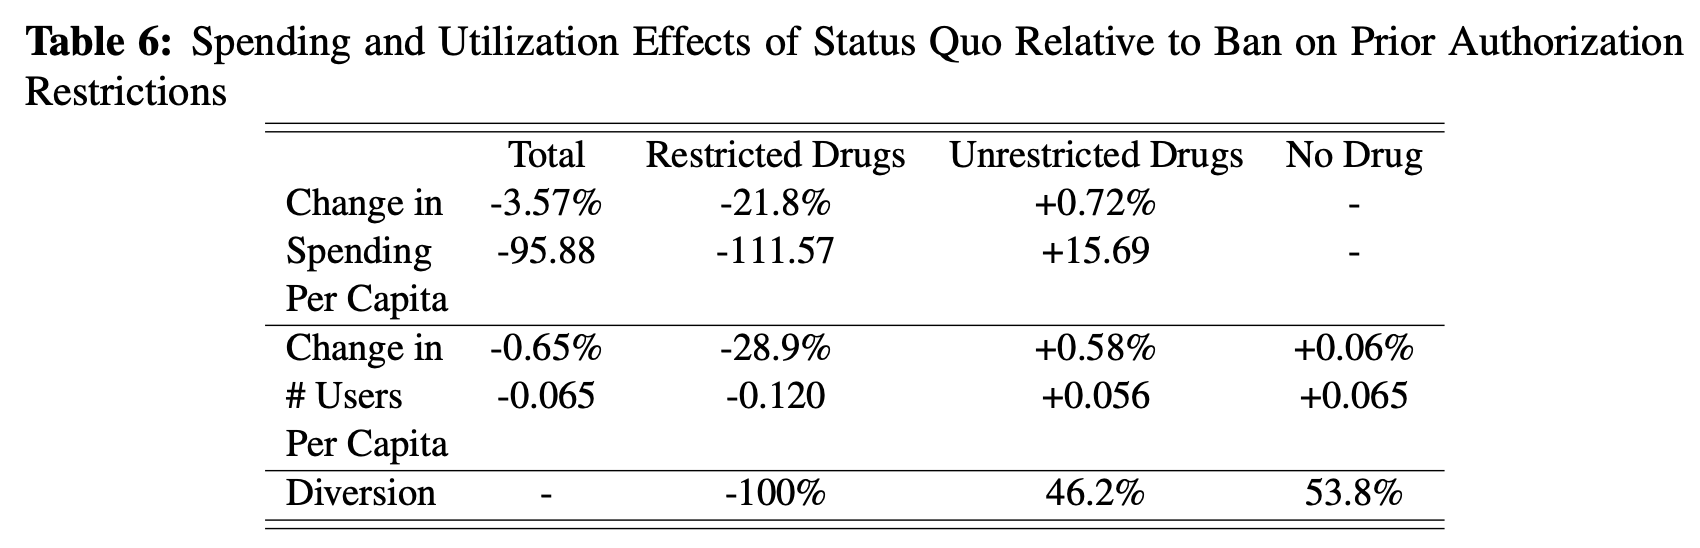
\includegraphics[width=0.8\linewidth]{tb6-spending-effect.png}
    \end{figure}
\end{frame}

\section{Administrative Cost Burdens}
\begin{frame}{Administrative Cost Burden}
    relevant parameters:
    \begin{itemize}
        \item joint cost to both the physician (submit requests) and the insurer (process requests): $a$
        \item constant rejection rate across all drugs and years: $r$
        \item \# of patients taking the drug: $N$
    \end{itemize}    
    then there will be $\frac{N}{1-r}$ requests and the administrative cost is $\frac{aN}{1-r}$ \\
\end{frame}
\begin{frame}{Administrative Cost Burden-- Calibration}
    \begin{itemize}
        \item estimates $N$ using simulation under status quo in the previous section
        \item estimates cost $a$ based on previous literature: provider-side paperwork cost is $\$ 18.53$ per application; processing cost is $\$ 3.95$ per application 
    \end{itemize}
    \begin{figure}
        \centering
        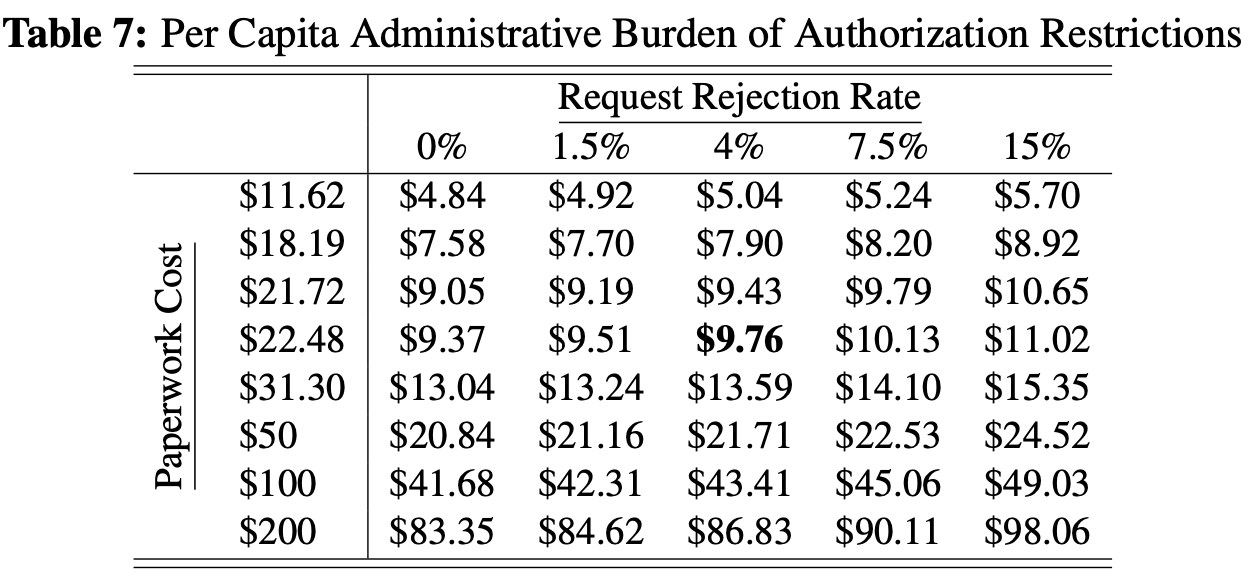
\includegraphics[width=0.7\linewidth]{tb7-admin-cost.png}
        \caption{subtracting from \$96, a net saving of around \$86 }
    \end{figure}
\end{frame}


\section{Welfare Effects}

\subsection{Revealed Preference Approach}
\begin{frame}{Welfare Effect: a Revealed Preference Approach}
    aim: estimate the total loss in consumer surplus due to being turned away from a drug
    $$\triangle CS_d = -\int_{\Theta_M} V_d(\theta) d\theta $$

    denote the WTP for drug $d$ for $\theta$ type consumer as $W_d(\theta_{id})$ \\
    the market demand curve is $D_d(P_d) =\int 1\{W_d(\theta) \geq P_d \}d \theta $ \\
    use the exogenous variation in $P_d$ to trace out $D_d (\cdot)$ and the distribution of $W_d$ \\
    if $W_d(\theta)=V_d(\theta)$, can get the distribution of $V_d$
\end{frame}
\begin{frame}{Welfare Effect: a Revealed Preference Approach}
    leverage the transitions of 62,785 beneficiaries into the LIS as a source of exogenous variation in price \\
    \begin{equation}
        \log(E[Y_{idt}])=\frac{\epsilon}{100}P_{dt}\times NotLIS_{it} + \alpha_i + \gamma_{dmt} + \epsilon_{it}
    \end{equation}
    where $P_{dt}\times NotLIS_{it}$ is equal to the price of the drug d in year t for those not yet enrolled in the LIS program ($NotLIS_it$ = 1) and zero for those enrolled ($NotLIS_it$ = 0) \\
    estimated by Poisson regression, the estimated $\epsilon = 0.15$ \\
    assume the demand curve is $D_d(P_d) = D_d(0)e^{\frac{\epsilon}{100}P_d}$
    then the distribution of $W_d$ is $$F_d(W)=1-D_d(0)e^{\frac{\epsilon}{100}W}$$
    estimate $D_d(0)$ in simulation absent of restriction
\end{frame}



\begin{frame}{Welfare Effect: a Revealed Preference Approach}
    for $W_d=V_d$, 
    \begin{itemize}
        \item if marginal beneficiaries screened away are those with the lowest WTP
        $$\triangle CS_d^{best-case} = -\int_{(1-0.289)D_d(0)}^{D_d(0)} D_d^{-1}(\theta) d\theta $$

        \item if screening is random
        $$\triangle CS_d^{random} = -0.289\int_0^{D_d(0)} D_d^{-1}(\theta) d\theta $$
        
    \end{itemize}
    
\end{frame}



\begin{frame}{Welfare Effect: a Revealed Preference Approach}
    \begin{figure}
        \centering
        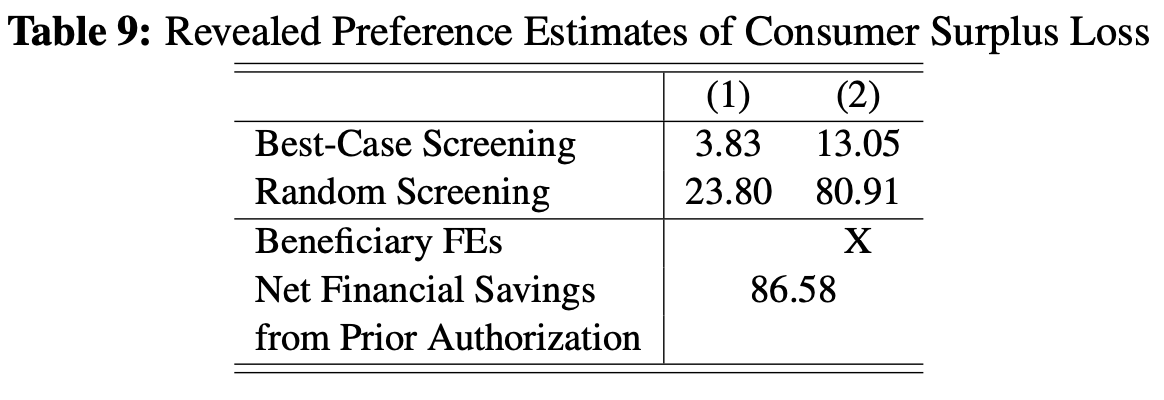
\includegraphics[width=0.75\linewidth]{tb9.png}
        \caption{two columns represent two amounts under the two estimates of semi-elasticity demand. Under the best-case screening, the amount consumers are willing to pay for the forgone drugs is around 15\% of the net savings. In the random screening case, the amount consumers are willing to pay for the forgone consumption is in the same general range as the net savings.}
        \label{fig:enter-label}
    \end{figure}
\end{frame}
% \begin{frame}{Welfare Effect: a Revealed Preference Approach}
    \begin{itemize}
        \item if WTP is not equivalent with value
        \item assume $W_d(\theta)=\rho V_d(\theta)$
        \item then $\triangle CS^{Debiased}=\frac{1}{\rho}\triangle CS^{Estimated}$ 
        \item the value of $\rho$ required to make prior authorization inefficient is 0.15  and 0.93 respectively, for the best-case and random scenarios.
    \end{itemize}
    
\end{frame}

\subsection{Health Effects}
\begin{frame}{Health Effects: Case Study of Oral Anticoagulants}
    understand the impact of prior authorization restrictions on access to non-Vitamin K oral anticoagulants (NOACs) compared to warfarin, a low-priced generic alternative, with:
    $$Y_{it}=\beta AuthAllNOACs_{j(it)t} + \gamma OtherFormulary_{j(it)t} + \delta_{m(it)} + \epsilon_{it} $$
    , where 
    \begin{itemize}
        \item $AuthAllNOACs$ is a dummy variable indicating whether assigned to a plan $j$ where all NOACs were restricted; 
        \item $Y$ is an indicator of a beneficiary’s health outcomes
    \end{itemize}
    health outcomes such as strokes, bleeding events, and death yield inconclusive results
\end{frame}
\begin{frame}{Health Effects: Aggregate Health Effects}
    construct two indicators:
    \begin{itemize}
        \item $AuthExposureQ5_i$ whether the beneficiary’s assigned plan was in the quantile with the most exposure to prior authorization
        \item $ExclExposureQ5_i$ assignment to the worst plans in terms of their exclusion of previously-taken drugs
    \end{itemize}
    $$Y_{it}=\beta AuthExposureQ5_i + \gamma ExclExposureQ5_i + \delta_{m(i)} + \epsilon_{i} $$
    
\end{frame}
\begin{frame}{Health Effects: Aggregate Health Effects}
    \begin{figure}
        \centering
        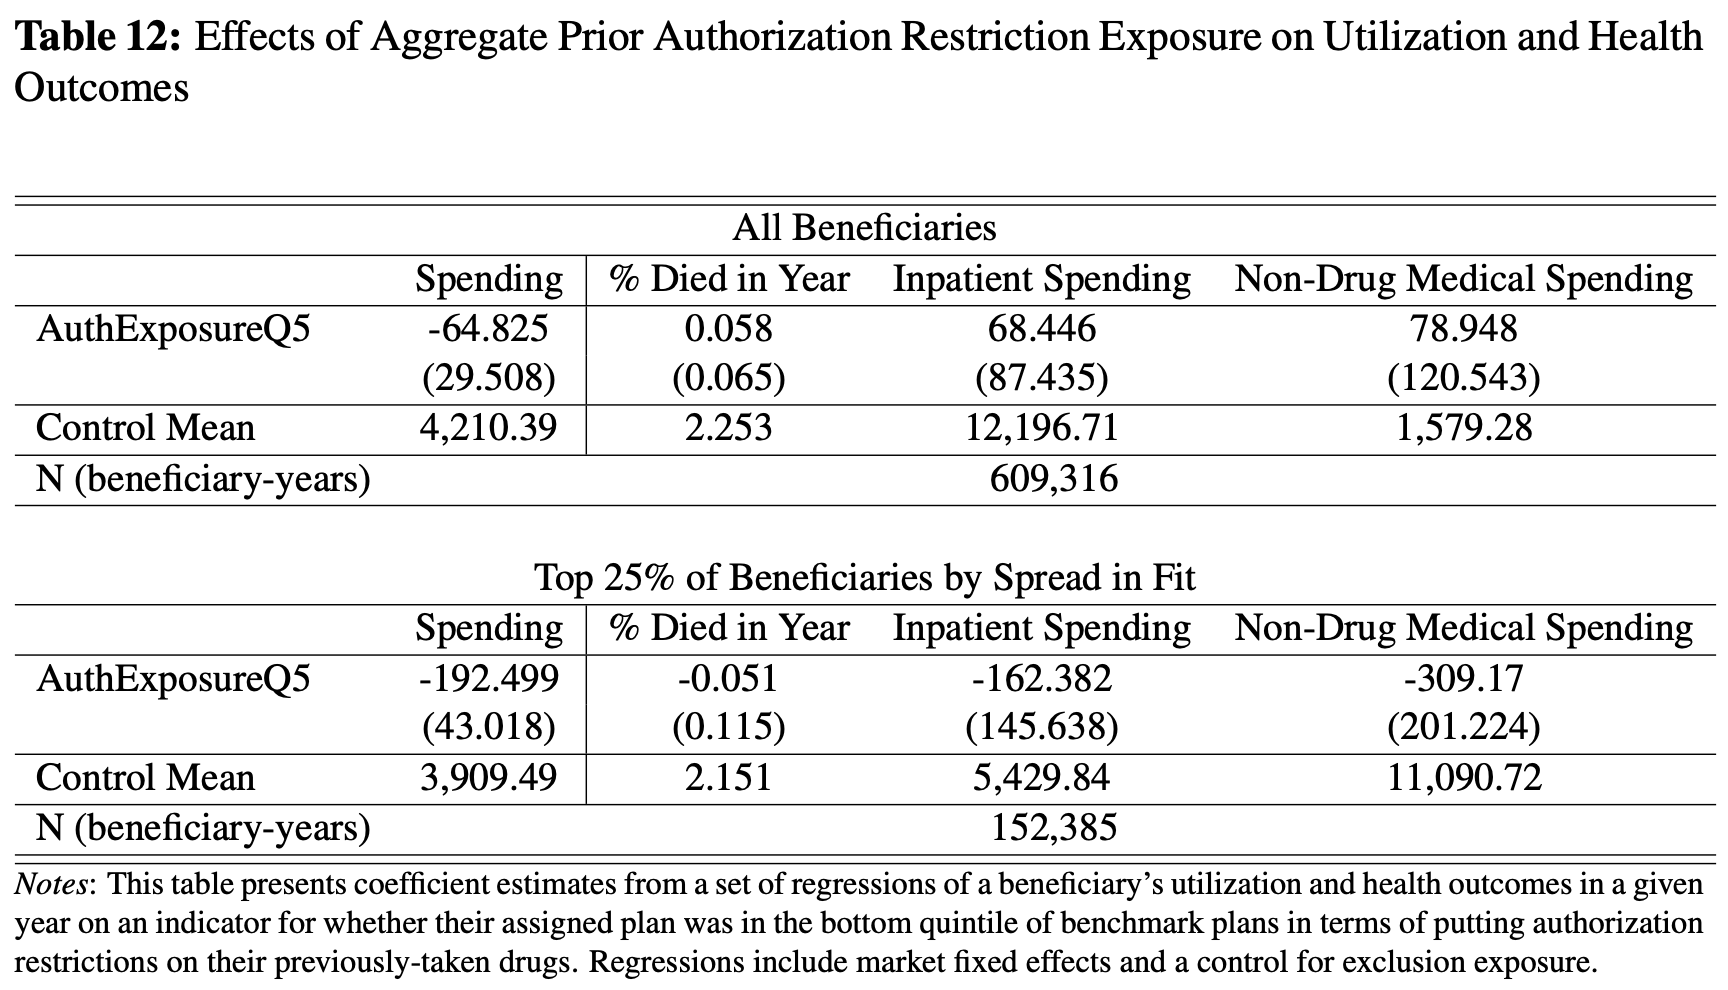
\includegraphics[width=0.75\linewidth]{tb12-health-effect.png}
        \caption{second panel restrict to a subset of beneficiaries who face the greatest variation across plans in terms of exposure to prior authorization}
    \end{figure}
\end{frame}

\section{Conclusion}
\begin{frame}{Conclusion}
    \begin{itemize}
        \item reducing drug spending by \$96 per beneficiary-year , while only generating approximately \$10 in paperwork costs. The cost savings likely exceed beneficiaries’ willingness to pay for foregone drugs.

        \item Despite its benefits, prior authorization policies may not be optimal if implemented more widely, and there may be more efficient alternatives for managing healthcare costs.
    \end{itemize}
\end{frame}

\end{document}